\documentclass{documentation}
\usepackage{tikz}
\usetikzlibrary{shapes.geometric, arrows}
\tikzstyle{module} = [rectangle, rounded corners, minimum width=3cm, minimum height=1cm,text centered, draw=black]
\tikzstyle{decision} = [diamond, minimum width=3cm, minimum height=1cm, text centered, draw=black, fill=green!30, aspect=2]
\usetikzlibrary{positioning, fit, calc, chains}

\title{Dokumentacja Techniczna Backend}

\author{Tomasz Chady}

\begin{document}

\maketitle

\tableofcontents

\newpage

\section{Dokumentacja API}

\subsection{Endpointy}

Dokumentacja endpointów jest dostępna w formacie OpenAPI 3.0.0.
Dostępna jest w \href{https://github.com/Stanlee77/ASSASSIN/blob/master/backend/openapi.yaml}{surowym formacie}, \href{https://github.com/Stanlee77/ASSASSIN/blob/master/doc/openapi.md}{reprezentacji Markdown} oraz na \href{https://stanlee77.github.io/ASSASSIN/openapi.html}{Github Pages}.
Dodatkowo wraz z backendem dostarczona jest dokumentacja w formacie Swagger UI pod ścieżką \codeword{\docs}.

\subsection{Autoryzacja}

Autoryzacja w systemie odbywa się na dwa sposoby.
Są one zdefiniowane w \href{https://github.com/Stanlee77/ASSASSIN/blob/master/backend/controllers/authController.js}{authController.js}.
Pierwszym sposobem jest autoryzacja poprzez hasło i login.
Drugim z nich to autoryzacja przez JWT token.
Autoryzacja poprzez hasło i login jest wykorzystywana do logowania się do systemu.
Metody autoryzacyjne są zdefiniowane w ramach Passport.js.
Dodawane są one do endpointów w zależności od potrzeb.

\subsubsection{Login}

Autoryzacja poprzez login i hasło jest wewnętrznie nazwana \codeword{login}.
Login i hasło są przesyłane w body requestu w formacie JSON.
Przykładowy request jest przedstawiony poniżej.

\begin{lstlisting}
...
"authInfo":{
    "login": "admin",
    "password": "admin"
}
...
\end{lstlisting}

\subsubsection{JWT}

Autoryzacja poprzez JWT token jest wewnętrznie nazwana \codeword{jwt}.
JWT token jest przesyłany w nagłówku \codeword{Authorization} w formacie \codeword{Bearer <token>}.
W systemie token JWT jest generowany po poprawnym zalogowaniu się do systemu.

\section{Architektura Backendu}

Backend został napisany w formie monolitycznego REST API.
Głównym zadaniem backendu jest udostępnienie danych z bazy danych.
Dodatkowo backend jest odpowiedzialny za interakcję z powiązanymi systemami oraz autoryzację użytkowników.
Relatywna pozycja backendu w systemie jest przedstawiona na schemacie \ref{fig:arch}.

\begin{figure}[h]
    \centering
    \includegraphics[width=0.8\textwidth]{Level_2_C4_Model.png}
    \caption{Schemat architektury\label{fig:arch}}
\end{figure}

Backend jest napisany w języku JavaScript z użyciem środowiska Node.js.
Aby zapewnić czytelność i łatwiejszy rozwój kod został podzielony na moduły w poszczególnych plikach i folderach.
Poniżej znajduje się lista modułów wraz z krótkim opisem.

\begin{itemize}
    \item \textbf{index.js} - główny plik aplikacji, zawiera konfigurację serwera, endpointów oraz uruchamia go.
    \item \textbf{env.js} - moduł odpowiedzialny za wczytanie zmiennych środowiskowych.
    \item \textbf{routes} - folder zawierający pliki z endpointami.
    \item \textbf{controllers} - folder zawierający pliki z kontrolerami.
    \item \textbf{services} - folder zawierający pliki z serwisami.
    \item \textbf{db} - folder zawierający pliki z modelami bazy danych.
\end{itemize}

Schemat zależności między modułami znajduje się na schemacie \ref{fig:dependency}.

\begin{figure}[h]
    \centering
    \scalebox{0.7}{
        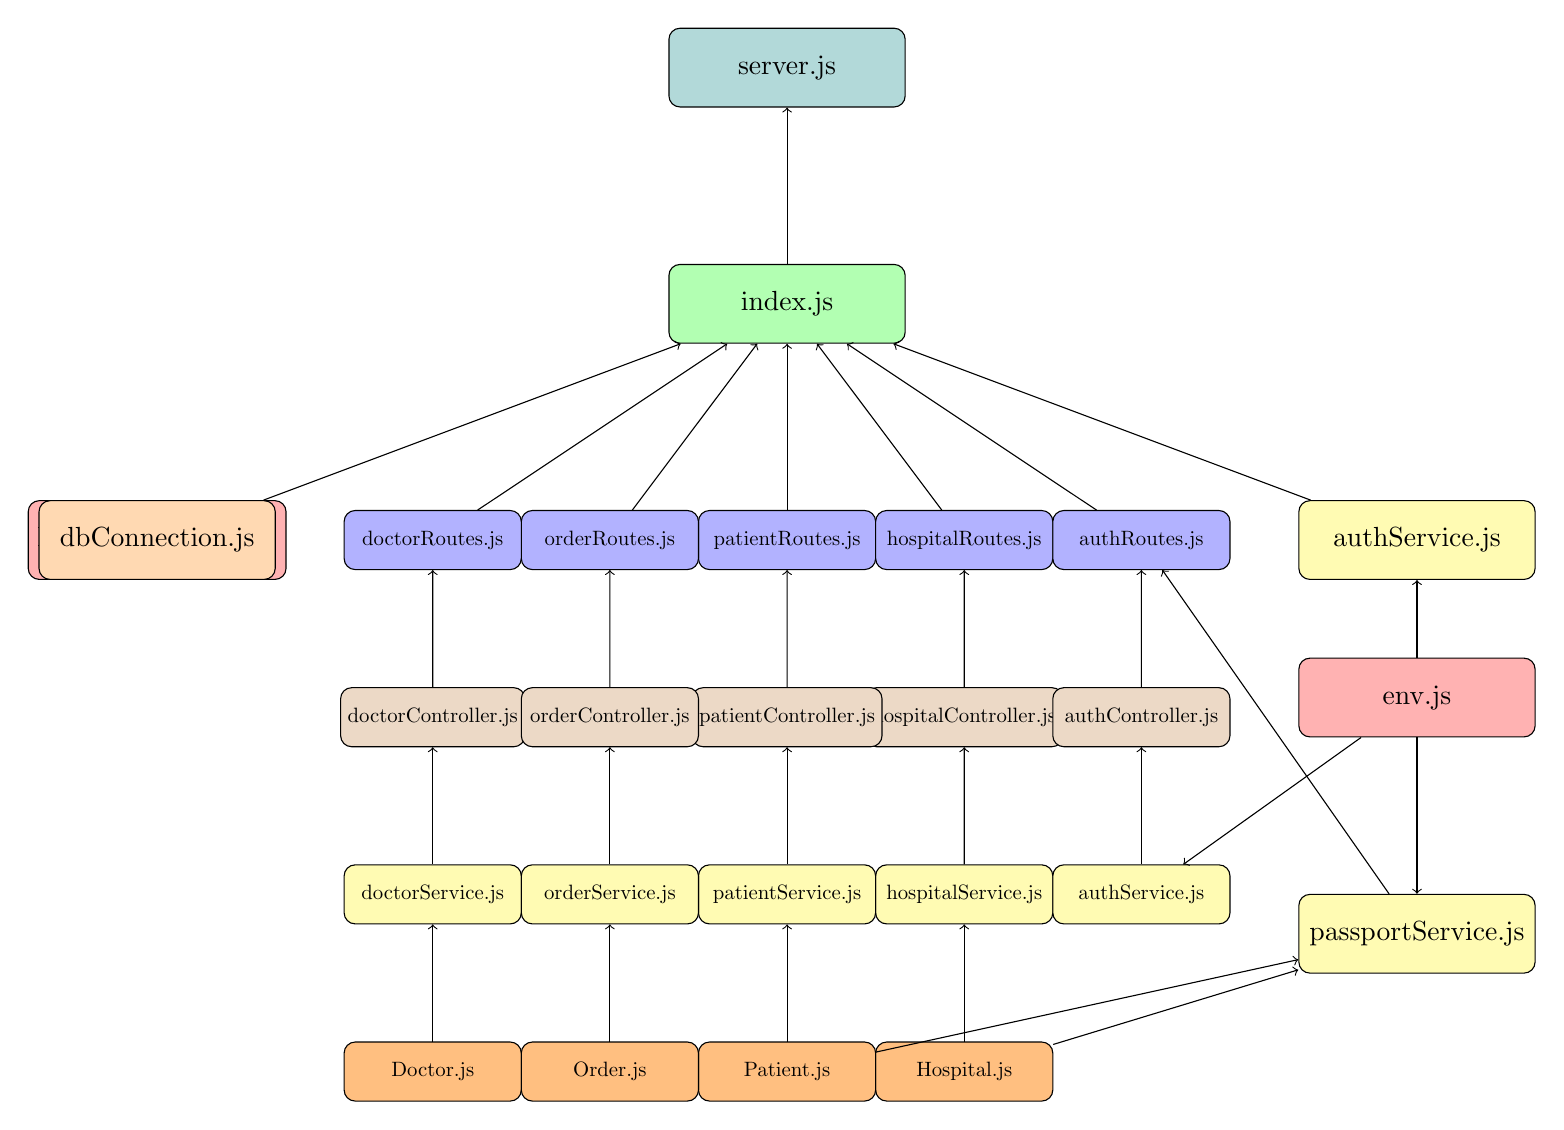
\begin{tikzpicture}[node distance=3cm]
            \tikzstyle{route} = [module, fill=blue!30, scale=0.75, node distance=3cm]
            \tikzstyle{controller} = [route, fill=brown!30]
            \tikzstyle{service} = [route, fill=yellow!30]
            \tikzstyle{dbModel} = [route, orange!50, text=black, draw=black]

            \node[module, fill=teal!30] (server) {server.js};
            
            \node[module, fill=green!30, below of=server] (index) {index.js};
            \node[module, fill=red!30, below of=index, xshift=-8cm] (logger) {loggerMiddleware.js};

            \node[module, fill=orange!30, below of=index, xshift=-8cm] (db) {dbConnection.js};
            
            \node[route, below of=index, yshift=-1cm] (patient) {patientRoutes.js};
            \node[route, right of=patient] (hospital) {hospitalRoutes.js};
            \node[route, right of=hospital] (authRoutes) {authRoutes.js};
            \node[route, left of=patient] (order) {orderRoutes.js};
            \node[route, left of=order] (doctor) {doctorRoutes.js};

            \node[controller, below of=hospital] (hospitalController) {hospitalController.js};
            \node[controller, below of=doctor] (doctorController) {doctorController.js};
            \node[controller, below of=patient] (patientController) {patientController.js};
            \node[controller, below of=order] (orderController) {orderController.js};
            \node[controller, below of=authRoutes] (authController) {authController.js};
            
            \node[service, below of=hospitalController] (hospitalService) {hospitalService.js};
            \node[service, below of=doctorController] (doctorService) {doctorService.js};
            \node[service, below of=patientController] (patientService) {patientService.js};
            \node[service, below of=orderController] (orderService) {orderService.js};
            \node[service, below of=authController] (authService) {authService.js};

            \node[dbModel, below of=hospitalService] (hospitalModel) {Hospital.js};
            \node[dbModel, below of=doctorService] (doctorModel) {Doctor.js};
            \node[dbModel, below of=patientService] (patientModel) {Patient.js};
            \node[dbModel, below of=orderService] (orderModel) {Order.js};
            
            \node[module, fill=yellow!30, below of=index, xshift=8cm] (auth) {authService.js};
            \node[module, fill=yellow!30, below of=auth, yshift=-2cm] (passportService) {passportService.js};
            \node[module, fill=red!30, below of=auth, xshift=0cm, yshift=1cm] (env) {env.js};

            \draw[->] (index) -- (server);
            \draw[->] (db) -- (index);
            \draw[->] (auth) -- (index);
            \draw[->] (env) -- (auth);
            \draw[->] (env) -- (authService);
            \draw[->] (env) -- (passportService);
            \draw[->] (passportService) -- (authRoutes);
            \draw[->] (patientModel) -- (passportService);
            \draw[->] (hospitalModel) -- (passportService);
            
            \draw[->] (hospital) -- (index);
            \draw[->] (doctor) -- (index);
            \draw[->] (authRoutes) -- (index);
            \draw[->] (patient) -- (index);
            \draw[->] (order) -- (index);

            \draw[->] (hospitalController) -- (hospital);
            \draw[->] (doctorController) -- (doctor);
            \draw[->] (authController) -- (authRoutes);
            \draw[->] (patientController) -- (patient);
            \draw[->] (orderController) -- (order);

            \draw[->] (hospitalService) -- (hospitalController);
            \draw[->] (doctorService) -- (doctorController);
            \draw[->] (authService) -- (authController);
            \draw[->] (patientService) -- (patientController);
            \draw[->] (orderService) -- (orderController);

            \draw[->] (hospitalModel) -- (hospitalService);
            \draw[->] (doctorModel) -- (doctorService);
            \draw[->] (patientModel) -- (patientService);
            \draw[->] (orderModel) -- (orderService);

        \end{tikzpicture}
    }
    \caption{Schemat wymagań\label{fig:dependency}}
\end{figure}

Bardzo dobrze widać na tym wykresie warstwowość architektury backendu.
Index.js wykorzystuje ścieżki zdefiniowane w routes do wywoływania odpowiednich funkcji zdefiniowanych w kontrolerach.
Z kolei kontrolery wykorzystują serwisy do wykonywania operacji na bazie danych.
Serwisy polegają na wywoływaniu odpowiednich funkcji zdefiniowanych w modelach bazy danych.

\indent Dokładniejszy schemat zależności między funkcjami, z perspektywy API znajduje się na schemacie \ref{fig:API}.
Przedstawiono na nim jakie sposoby autentykacji są wykorzystywane w poszczególnych ścieżkach.
Ilość endpointów jest za duża aby je wszystkie przedstawić na schemacie.

\begin{figure}[h]
    \centerfloat
    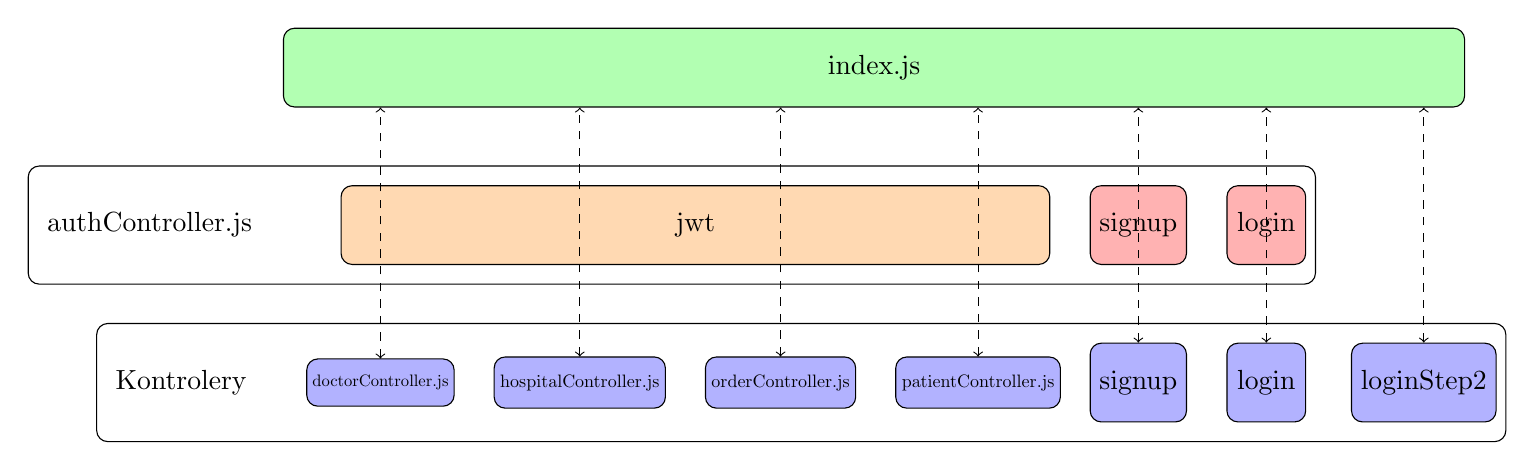
\begin{tikzpicture}[node distance=2cm, start chain=1 going right, start chain=2 going right]
        \tikzstyle{container} = [module, minimum height=1.5cm, minimum width=12cm]
        \tikzstyle{controller} = [module, minimum width=1cm, fill=blue!30]
        
        \node[module, fill=green!30, minimum width=15cm] (index) {index.js};
        
        \node[on chain=1, below of=index, xshift=-9.2cm] (authLabel) {authController.js};
        \node[module, fill=orange!30, minimum width=9cm, on chain=1, xshift=-1cm] (jwt) {jwt};
        \node[module, fill=red!30, minimum width=1cm, on chain=1, xshift=-1.5cm] (signup) {signup};
        \node[module, fill=red!30, minimum width=1cm, on chain=1, xshift=-1.5cm] (login) {login};
        \node[container, fit={(authLabel) (jwt) (signup) (login)}] (authBox) {};

        \node[below of=authLabel, xshift=0.4cm] (containerLabel) {Kontrolery};
        \node[controller, below of=jwt, xshift=-4cm, on chain=2, scale=0.6] (profile) {doctorController.js};
        \node[controller, on chain=2, xshift=-1.5cm, scale=0.65] (disable2fa) {hospitalController.js};
        \node[controller, on chain=2, xshift=-1.5cm, scale=0.65] (generate2faSecret) {orderController.js};
        \node[controller, on chain=2, xshift=-1.5cm, scale=0.65] (verifyOtp) {patientController.js};
        \node[controller, below of=signup] (signupFunc) {signup};
        \node[controller, below of=login] (loginFunc) {login};
        \node[controller, right of=loginFunc] (loginStep2) {loginStep2};
        \node[container, fit={(profile) (signupFunc) (loginFunc) (loginStep2) (disable2fa) (generate2faSecret) (verifyOtp) (containerLabel)}] (components) {};

        \draw[<->, dashed] (profile) -- (profile|-index.south);
        \draw[<->, dashed] (disable2fa) -- (disable2fa|-index.south);
        \draw[<->, dashed] (generate2faSecret) -- (generate2faSecret|-index.south);
        \draw[<->, dashed] (verifyOtp) -- (verifyOtp|-index.south);
        \draw[<->, dashed] (signupFunc) -- (signupFunc|-index.south);
        \draw[<->, dashed] (loginFunc) -- (loginFunc|-index.south);
        \draw[<->, dashed] (loginStep2) -- (loginStep2|-index.south);

    \end{tikzpicture}
    \caption{Schemat architektury wewnętrznej API\label{fig:API}}
\end{figure}

\section{Ścieżki}

W systemie istnieje kilka sekwencji operacji odpowiedzialnych za różne operacje.
Kilka z nich jest przedstawionych poniżej.

\begin{figure}[h]
    \centering
    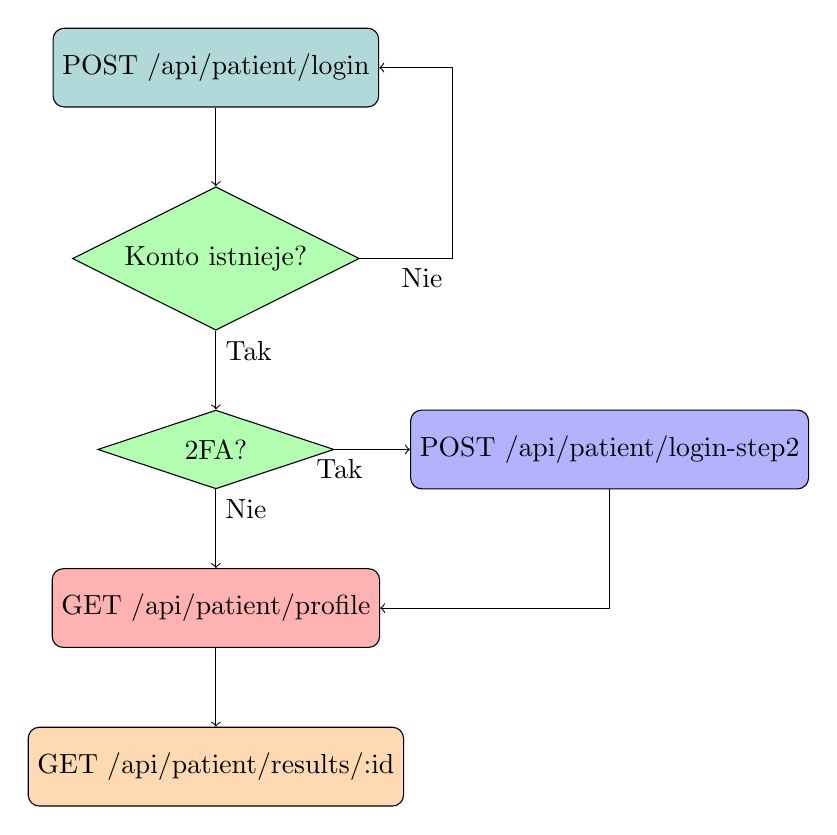
\begin{tikzpicture}[start chain=1 going below]
        \node[module, fill=teal!30, on chain] (login) {POST /api/patient/login};
        \node[decision, on chain] (account) {Konto istnieje?};
        \node[decision, on chain] (2fa) {2FA?};
        \node[module, fill=blue!30, right of=2fa, xshift=4cm] (loginStep2) {POST /api/patient/login-step2};
        \node[module, fill=red!30, on chain] (profile) {GET /api/patient/profile};
        \node[module, fill=orange!30, on chain] (order) {GET /api/patient/results/:id};

        \draw[->] (login) -- (account);
        \draw[->] (account) -- node[anchor=south west] {Tak} (2fa);
        \draw[->] (account.east) -| node[anchor=north east] {Nie} (3, -1) |-  (login.east);
        \draw[->] (2fa) -- node[anchor=north east] {Tak} (loginStep2);
        \draw[->] (2fa) -- node[anchor=south west] {Nie} (profile);
        \draw[->] (loginStep2) |- (profile);
        \draw[->] (profile) -- (order);
    \end{tikzpicture}
    \caption{Schemat wyświetlania wyników\label{fig:dataOutput}}
\end{figure}

\begin{figure}[h]
    \centering
    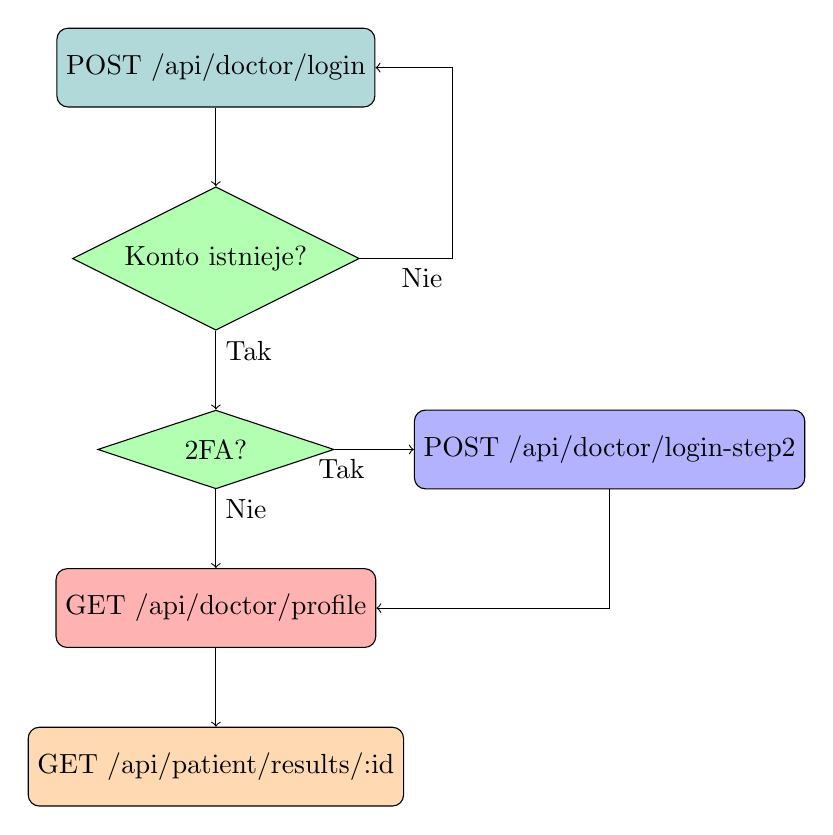
\begin{tikzpicture}[start chain=1 going below]
        \node[module, fill=teal!30, on chain] (login) {POST /api/doctor/login};
        \node[decision, on chain] (account) {Konto istnieje?};
        \node[decision, on chain] (2fa) {2FA?};
        \node[module, fill=blue!30, right of=2fa, xshift=4cm] (loginStep2) {POST /api/doctor/login-step2};
        \node[module, fill=red!30, on chain] (profile) {GET /api/doctor/profile};
        \node[module, fill=orange!30, on chain] (order) {GET /api/patient/results/:id};

        \draw[->] (login) -- (account);
        \draw[->] (account) -- node[anchor=south west] {Tak} (2fa);
        \draw[->] (account.east) -| node[anchor=north east] {Nie} (3, -1) |-  (login.east);
        \draw[->] (2fa) -- node[anchor=north east] {Tak} (loginStep2);
        \draw[->] (2fa) -- node[anchor=south west] {Nie} (profile);
        \draw[->] (loginStep2) |- (profile);
        \draw[->] (profile) -- (order);
    \end{tikzpicture}
    \caption{Schemat wyświetlania wyników przez lekarza\label{fig:dataOutputDoc}}
\end{figure}

\section{Baza danych}

Do projektu został wybrany silnik bazodanowy Mongoose.db.
Jest to silnik bazodanowy napisany w języku JavaScript, który działa na silniku MongoDB.
MongoDB jest bazą danych typu NoSQL, która przechowuje dane w formacie JSON.
Dzięki temu można w łatwy sposób przechowywać dane w formacie JSON, a także w łatwy sposób je przetwarzać.
Moduł odpowiedzialny za połączenie z bazą danych to \href{https://github.com/Stanlee77/ASSASSIN/blob/master/backend/db/dbConnection.js}{dbConnection.js}.

\subsection{Schemat}

Schemat bazy danych jest przedstawiony na schemacie \ref{fig:db}.

\begin{figure}[h!]
    \centering
    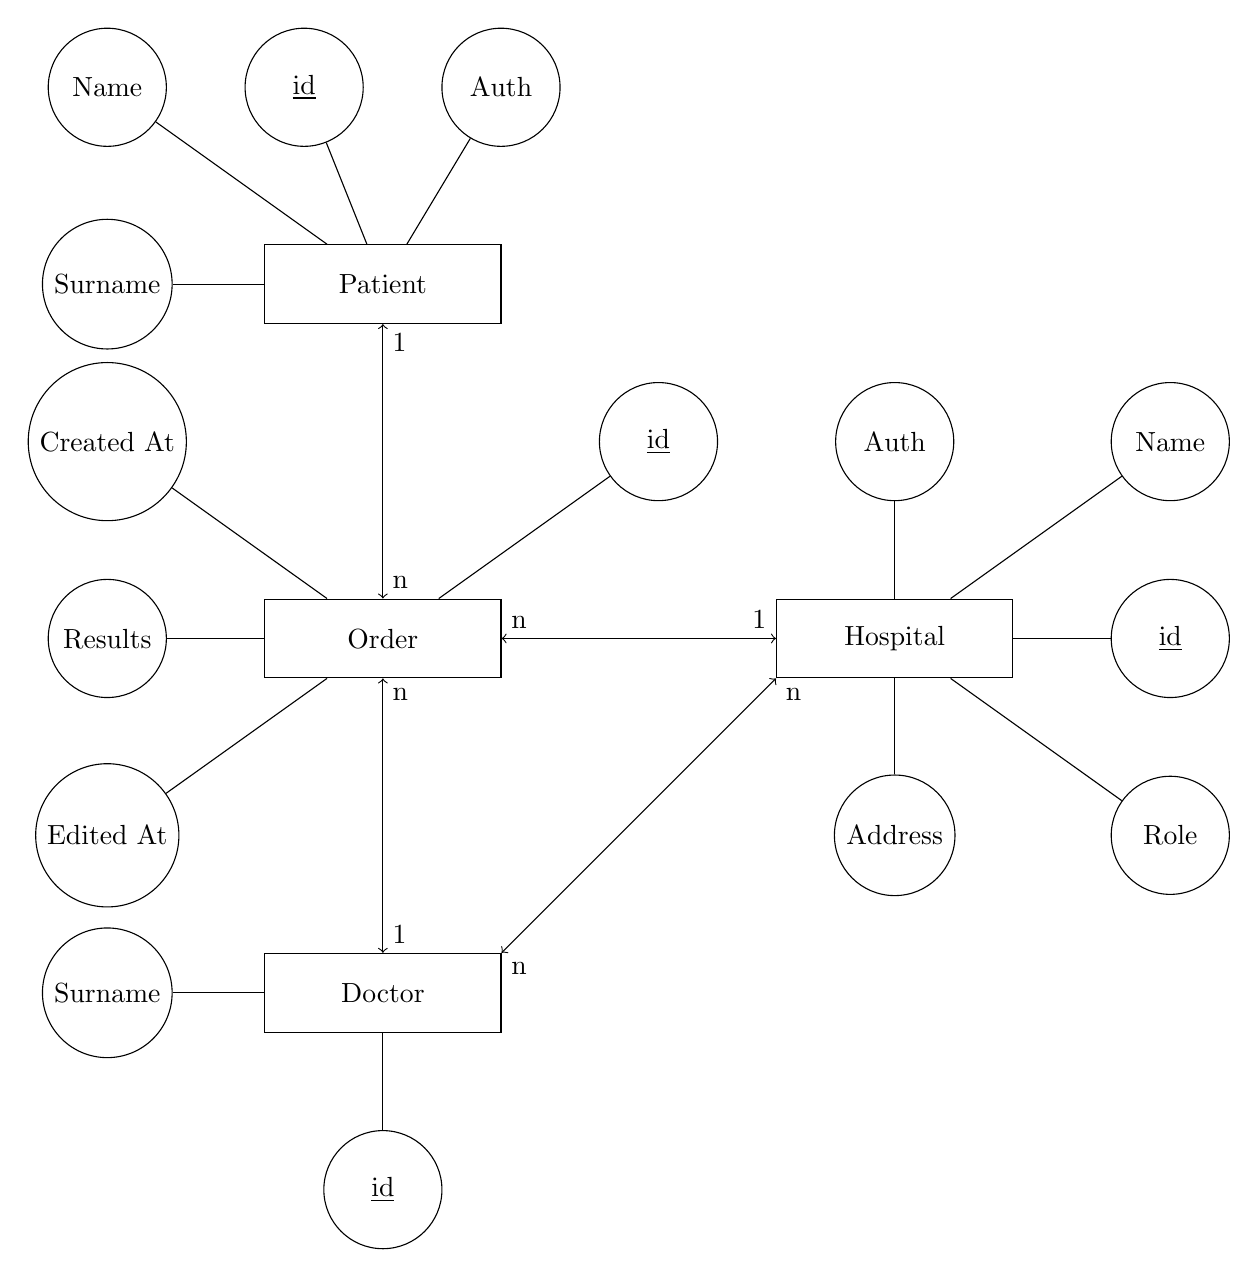
\begin{tikzpicture}[node distance=2.5cm]
        \tikzstyle{table} = [rectangle, minimum width=3cm, minimum height=1cm,text centered, draw=black]
        \tikzstyle{parameter} = [circle, minimum width=1.5cm, minimum height=1cm,text centered, draw=black]
        \node[table] (patient) {Patient};
        \node[parameter, left of=patient, xshift=-1cm] (surname) {Surname};
        \node[parameter, above of=surname] (name) {Name};
        \node[parameter, right of=name] (patientId) {\underline{id}};
        \node[parameter, right of=patientId] (pass) {Auth};

        \node[table, below of=patient, yshift=-2cm] (order) {Order};
        \node[parameter, left of=order, xshift=-1cm] (results) {Results};
        \node[parameter, below of=results] (editedAt) {Edited At};
        \node[parameter, above of=results] (createdAt) {Created At};
        \node[parameter, right of=order, yshift=2.5cm, xshift=1cm] (orderId) {\underline{id}};


        \node[table, below of=order, yshift=-2cm] (doctor) {Doctor};
        \node[parameter, left of=doctor, xshift=-1cm] (doctorSurname) {Surname};
        \node[parameter, below of=doctor] (doctorId) {\underline{id}};

        \node[table, right of=order, xshift=4cm] (hospital) {Hospital};
        \node[parameter, right of=hospital, xshift=1cm] (hospitalId) {\underline{id}};
        \node[parameter, above of=hospitalId] (hospitalName) {Name};
        \node[parameter, below of=hospitalId] (hospitalRole) {Role};
        \node[parameter, above of=hospital] (hospitalAuth) {Auth};
        \node[parameter, below of=hospital] (hospitalAddress) {Address};

        \draw[-] (patient) -- (name);
        \draw[-] (patient) -- (surname);
        \draw[-] (patient) -- (patientId);
        \draw[-] (patient) -- (pass);

        \draw[-] (order) -- (results);
        \draw[-] (order) -- (editedAt);
        \draw[-] (order) -- (createdAt);
        \draw[-] (order) -- (orderId);

        \draw[-] (doctor) -- (doctorSurname);
        \draw[-] (doctor) -- (doctorId);

        \draw[-] (hospital) -- (hospitalId);
        \draw[-] (hospital) -- (hospitalName);
        \draw[-] (hospital) -- (hospitalRole);
        \draw[-] (hospital) -- (hospitalAuth);
        \draw[-] (hospital) -- (hospitalAddress);
        
        %1-n patient-order
        \draw[<->] (patient) -- (order);
        \node[anchor=north west] at (patient.south) {1};
        \node[anchor=north west] at (order.south) {n};

        %1-n doctor-order
        \draw[<->] (doctor) -- (order);
        \node[anchor=south west] at (doctor.north) {1};
        \node[anchor=south west] at (order.north) {n};

        %1-n hospital-order
        \draw[<->] (hospital) -- (order);
        \node[anchor=south east] at (hospital.west) {1};
        \node[anchor=south west] at (order.east) {n};

        %n-n hospital-doctor
        \draw[<->] (hospital.south west) -- (doctor.north east);
        \node[anchor=north west] at (hospital.south west) {n};
        \node[anchor=north west] at (doctor.north east) {n};
    \end{tikzpicture}
    \caption{Schemat bazy danych\label{fig:db}}
\end{figure}

\subsection{Modele}

W systemie funkcjonują 4 modele danych.
Są to \codeword{Doctor}, \codeword{Patient}, \codeword{Hospital} oraz \codeword{Order}.
Zdefiniowane są one w formacie JSON i są przedstawione poniżej.

\subsubsection{Order}

Model order reprezentuje wynik badania.
Jest on przypisany do konkretnego szpitala, pacjenta oraz doktora.
Zawiera on również informacje o dacie wykonania badania oraz o wyniku.

\begin{lstlisting}[language=JavaScript]
{
    id: mongoose.Schema.Types.ObjectId,
    hospital: {
        type: mongoose.Schema.Types.ObjectId,
        ref: 'Hospital',
        required: true,
    },
    doctor: {
        type: mongoose.Schema.Types.ObjectId,
        ref: 'Doctor',
        required: true,
    },
    patient: {
        type: mongoose.Schema.Types.ObjectId,
        ref: 'Patient',
        required: true,
    },
    createdAt: {
        type: Date,
        default: Date.now,
    },
    editedAt: Date,
    results: {
        wbc: String,
        rbc: String,
        hct: String,
        mcv: String,
        mch: String,
        plt: String,
        mpv: String,
        rdw: String,
        pdw: String,
        hemoglobin: String,
    }
}
\end{lstlisting}

\subsubsection{Doctor}

Model doctor reprezentuje lekarza.
Lekarz ma przypisane szpitale oraz nazwisko.

\begin{lstlisting}[language=JavaScript]
{
    id: mongoose.Schema.Types.ObjectId,
    surname: String,
    hospitals: [{
        type: mongoose.Schema.Types.ObjectId,
        ref: 'Hospital',
    }]
}
\end{lstlisting}

\subsubsection{Patient}

Model patient reprezentuje pacjenta.
Pacjent ma przypisane wyniki badań, i co za tym idzie pośrednio ma przypisane szpitale.

\begin{lstlisting}[language=JavaScript]
{
    name: String,
    surname: String,
    authInfo: {
        login: {
            type: String,
            required: true,
            unique: true,
        },
        password: {
            type: String,
            required: true,
        },
    },
    twofaEnabled: {
        type: Boolean,
        default: false,
    },
    twofaSecret: {
        type: String,
        default: "",
    },
    orders: [{
        type: mongoose.Schema.Types.ObjectId,
        ref: 'Order',
    }]
}
\end{lstlisting}

\subsubsection{Hospital}

Model hospital reprezentuje szpital.
Szpital jest powiązany z lekarzami oraz badaniami.
Dodatkowo szpital ma przypisane dane autoryzacyjne.

\begin{lstlisting}[language=JavaScript]
{
    id: mongoose.Schema.Types.ObjectId,
    name: String,
    role: {
        type: String,
        validate: {
            validator: function (value) {
                return value === 'hospital';
            },
            message: 'Role must be "hospital"',
        },
    },
    authInfo: {
        login: String,
        password: String,
    },
    orders: [{
        type: mongoose.Schema.Types.ObjectId,
        ref: 'Order',
    }],
    doctors: [{
        type: mongoose.Schema.Types.ObjectId,
        ref: 'Doctor',
    }],
    address: {
        street: String,
        zipCode: String,
        city: String,
    },
    twofaEnabled: {
        type: Boolean,
        default: false,
    },
    twofaSecret: {
        type: String,
        default: "",
    }
}
\end{lstlisting}

\end{document}